\documentclass[dvipdfmx,8pt]{beamer}
\usepackage{bxdpx-beamer}
\usepackage{pxjahyper}
\renewcommand{\kanjifamilydefault}{\gtdefault}
% \usetheme{metropolis}
\title{The Elements of Statistical Learning\\Chap.10: Boosting and Additive Tree}
\date{\today}
\author{Kosuke Kito}
\begin{document}
  \maketitle
  \begin{frame}{流れ}
    \begin{itemize}
      \item ``AdaBoost.M1''の話
      \item BoostingとAdditive Modelの相性がいい話
      \item Forward Stagewise(Additive Modelで使える計算方法)の話
      \item 損失関数の話
      \item Data Mining における手法の``実用性''の話
      \item 木を使ったBoostingの話
      \item 勾配Boostingの話
      \item 正則化の話
      \item 計算結果の解釈の話
    \end{itemize}
  \end{frame}
  \section{``AdaBoost.M1''の話\\p.337-}
  \begin{frame}{Boostingとは?ざっくりと. }
    \begin{itemize}
      \item ``弱い''分類器を組み合わせて使うことで, 効果的な分類を行う手法.
      \item この元になる 分類器たちのことを``base learner''と呼ぶ.
      \item 元々は分類用に考えられた. 今は回帰にも応用されている.
      \item baggingとの違いは, 前の手順の推定結果が次の手順に影響するかしないか. (袋から球を取り出した後, 戻すか戻さないかのイメージ?)
      \item 例として, Boostingで一番有名な``AdaBoost.M1''というアルゴリズムを紹介するよ.
    \end{itemize}
  \end{frame}
  \begin{frame}{AdaBoost.M1}
    \begin{columns}[t]
      \begin{column}{0.5\linewidth}
        \begin{itemize}
          \item 2クラスへの分類問題用のアルゴリズム. (当面は2クラスの分類問題しか考えません. が, 多値分類や回帰にも自然に拡張できる感じです. )
          \item 各$G_m \ (m=1,\dots,M)$は, 弱い分類器. つまり, $\{-1,1\}$への関数で, 正解率がランダムよりは多少良いもの.
          \item それまでの手順で正しく分類できなかったデータ程, 重視される. (画像の2-(d))
          \item 最後に合算するときは, 正答率の高かった時の推定が重視される(画像の3)
          \item 各分類器の値域が離散値なので, ``Discrete AdaBoost''とも.
          \item 値域を連続値$[-1,1]$に変更して, 確率の推定に使うこともできる.
        \end{itemize}
      \end{column}
      \begin{column}{0.5\linewidth}
        \begin{figure}[htb]
          \centering
          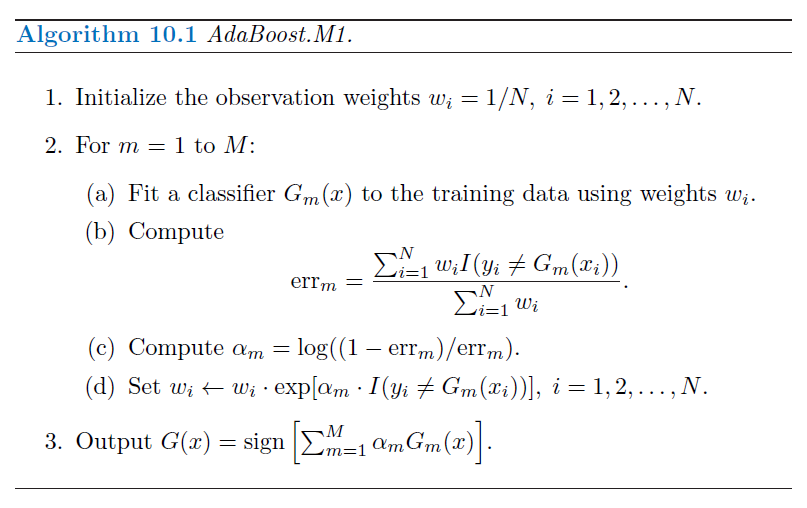
\includegraphics[width=5cm,clip]{images/AdaBoost.png}
        \end{figure}
      \end{column}
    \end{columns}
  \end{frame}
  \begin{frame}{AdaBoost.M1}
    \begin{figure}[htb]
      \centering
      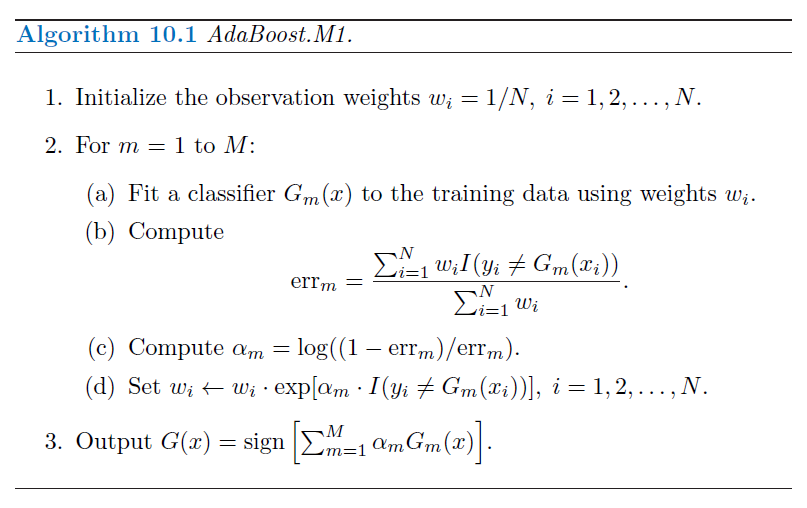
\includegraphics[width=8cm,clip]{images/AdaBoost.png}
    \end{figure}
  \end{frame}
  \begin{frame}{Boostingすごいぞ}
    \begin{columns}[t]
      \begin{column}{0.5\linewidth}
        \begin{itemize}
          \item 用語. ``Stump''とは, 単純な2分類の分類木.
          \item もちろん, とても弱い分類器.
          \item でも, これでBoostingすると, 244分類の分類木よりも良い性能を出せる.
        \end{itemize}
      \end{column}
      \begin{column}{0.5\linewidth}
        \begin{figure}[htb]
          \centering
          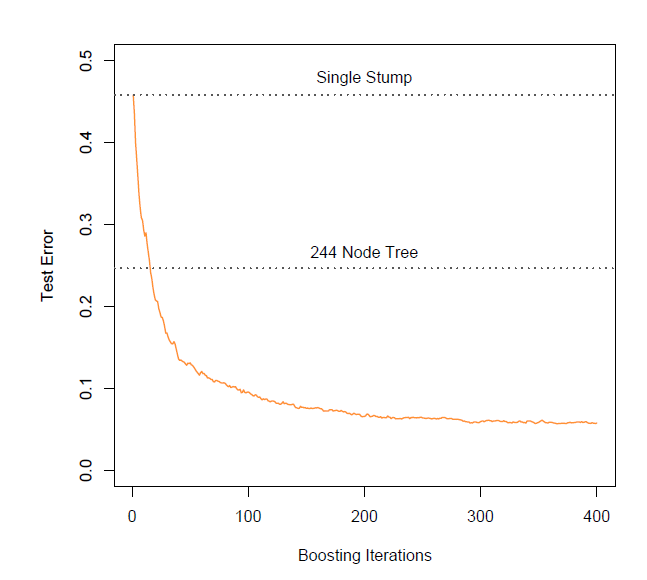
\includegraphics[width=5cm,clip]{images/StumpBoosting.png}
        \end{figure}
      \end{column}
    \end{columns}
  \end{frame}
  \section{BoostingとAdditive Modelの相性がいい話\\p.341-}
  \begin{frame}{BoostingとAdditive Model}
    AdaBoostの最後の式とAdditive Modelの式は似ている.
    \begin{itemize}
      \item AdaBoostの最後の式
        \[
          G(x)=\mathrm{sign}\left ( \sum_{m=1}^{M}\alpha_{m}G_{m}(x) \right )
        \]
      \item Additive Modelの式
        \[
          f(x)=\sum_{m=1}^{M}\beta_{m}b(x; \gamma_{m})
        \]
    \end{itemize}

    → Boostingは, base learnerを使った加法的な基底関数展開と思える.

    こんな感じで, Additive Modelの特殊な例と思えるものが, この本の中には多い.
  \end{frame}
  \section{Forward Stagewise(Additive Modelで使える計算方法)の話\\p.342-}
  \begin{frame}{Additive Modelの最適化}
    Additive Modelの最適化は, 損失関数を適当にとって, 損失の合計を最小化しようとすることが多い.
    \[
      \min_{\{\beta_{m},\gamma_{m}\}_{m=1}^{M}}\sum_{i=1}^{N}L\left ( \sum_{m=1}^{M}\beta_{m}b(x; \gamma_{m}) \right )
    \]
    ただし, 計算量が凄いことになるので, 困る. そこで出てくるのが, ``Forward Stagewise Additive Modeling''.
  \end{frame}
  \begin{frame}{Forward Stagewise Additive Modeling}
    \begin{columns}[t]
      \begin{column}{0.5\linewidth}
        \begin{itemize}
          \item いわゆる, 貪欲法(Greedy algorithm).
          \item 各基底関数ごとの最適化は簡単なときに有効.
          \item 前から一個ずつそこまでの結果との和を使って最適化していく.
          \item Squared-error loss
            \[
              L(y,f(x))=(y-f(x))^{2}
            \]
            に代表される, 残差にのみ依存する損失関数の場合, 残差に向かう最適化と思っても同義.
        \end{itemize}
        (ちなみに, Squared-errorは, 分類のための損失関数として良い選択肢じゃないよ. ちょっと後で考える. )
      \end{column}
      \begin{column}{0.5\linewidth}
        \begin{figure}[htb]
          \centering
          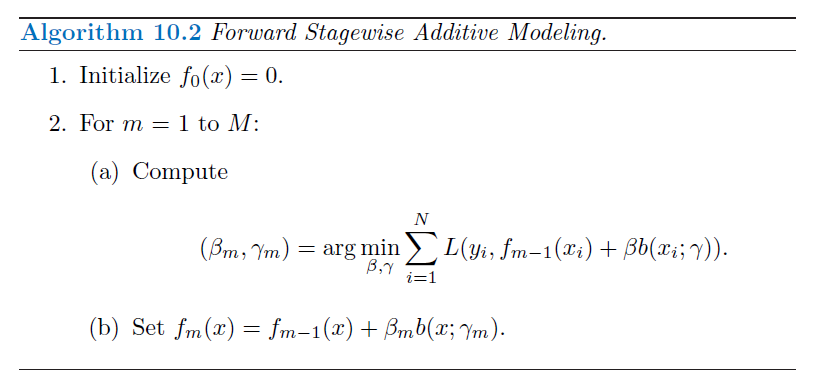
\includegraphics[width=5cm,clip]{images/ForwardStagewise.png}
        \end{figure}
      \end{column}
    \end{columns}
  \end{frame}
  \section{損失関数の話\\p.343-}
  \begin{frame}{Forward StagewiseとAdaBoost}
    \begin{itemize}
      \item AdaBoost.M1は, 損失関数として以下を使ったForward Stagewise Additive Modelingと思える.
        \[
          L(y,f(x))=e^{-yf(x)}
          \]
      \item 証明は割愛. 結構単純な計算なので, やってみるとよいかも?
      \item 損失関数として, これを採用する理由については後述.
      \item ちなみに, AdaBoostは, Forward Stagewiseとは全然別に考えられて, 後から一緒やん, ってなったらしいです.
    \end{itemize}
  \end{frame}
  \begin{frame}{指数損失関数を使うことの正当化}
    \begin{itemize}
      \item 指数損失関数の強みの一つは, 計算が簡単なこと. AdaBoostの反復計算の重みの更新はとても単純.
      \item 一方, 統計的にも良い. 指数損失関数の''Population Minimizer''は, ``Deviance''のそれと一致し, 母集団における事後確率になる.
      \item 用語. ``Population Minimizer''とは, パラメータ付きの確率分布から実数への関数を最小化するパラメータの値. 前に送った, 平均値・中央値・最頻値の話が非常に良い例になっている.

      例えば, 平均値は, 期待二乗誤差の``Population Minimizer''である, と言える.
      \item 用語. ``Deviance''とは, $-\log(\mbox{尤度})$で定まる値であり, 最尤法の損失関数と思える関数である. (たぶん, 結構バックグラウンドの分厚い概念だと思うのですが, あまり把握しきれず. )

      Binimial Deviance(2値分類におけるDeviance)は, 以下の式で定まる.
      \[
        \log \left ( 1+e^{-2Yf(x)} \right )
      \]
    \end{itemize}
  \end{frame}
  \begin{frame}{指数損失関数を使うことの正当化}
    \begin{itemize}
      \item 再び, 2個目の視点に戻る. 指数損失関数の"Population Minimizer"は,
      実際, 指数損失関数を使って最適化した式を$f^{*}(x)$とすると,
      \[
        f^{*}(x)=\mathrm{arg}\min_{f}\mathrm{E}_{Y \mid x}[e^{-Yf(x)}]=\frac{1}{2}\log\frac{\mathrm{P}[Y=1\mid x]}{\mathrm{P}[Y=-1\mid x]}
      \]
      となることが容易に分かる. もちろん, ``Deviance''を最小化するものは, 尤度を最大化するものなので, これは事後確率になって, 一致すると分かる.
      \item ちなみに, 上の式から, AdaBoostの最後に$\mathrm{sgn}$関数を使うことも納得.
      \item まとめると, 計算が楽(前節より)で, 最尤法と同じような答えが期待できるので, 指数損失関数はいいんじゃないか, という話.
    \end{itemize}
  \end{frame}
  \begin{frame}{損失関数と頑健さ}
    様々な損失関数を, 分類と回帰のそれぞれの場合について, ``頑健さ''(robustness)の視点から特徴づける.

    頑健さ, とは, 訓練データに異常値が含まれているときに, それに影響を受けにくい度合いのこと.
    ``noisy''な状況, つまり, 測定の質が低いときや, 母集団の分散が大きいときに, 頑健さが発揮される.

    損失関数の頑健さは, $y$と$f(x)$の値が離れるときの損失関数の値の大きくなる早さで評価できる.
  \end{frame}
  \begin{frame}{分類における頑健さ}
    \begin{columns}[t]
      \begin{column}{0.5\linewidth}
        \begin{itemize}
          \item 2値(-1/1)分類では, 回帰における残差の代わりに積$yf(x)$を採用できる.
          \item 誤分類は不連続な2値関数. 他は誤分類を扱いやすく連続にしようとしているものと思える.
          \item 母集団全体について考えると, 指数損失関数とDevianceは同じ推定をするが, 有限の訓練データに対しては異なる. $yf << 0$の時, 指数損失関数は指数関数的に増加するが, Devianceは線形であり, Devianceの方が頑健であるといえる.

          実際, AdaBoostはnoisyな状況ではパフォーマンスが大幅に悪化するらしい.
        \end{itemize}
        ちなみに, ここら辺の損失関数たちとかは, 自然と多値分類問題に拡張できます.
      \end{column}
      \begin{column}{0.5\linewidth}
        \begin{figure}[htb]
          \centering
          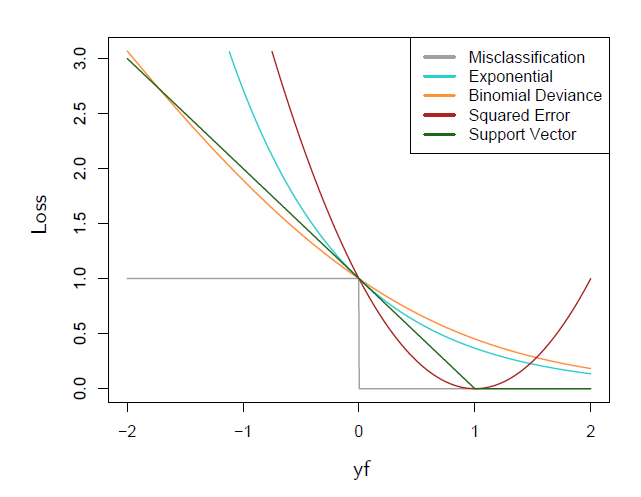
\includegraphics[width=5cm,clip]{images/RobustnessClassification.png}
        \end{figure}
      \end{column}
    \end{columns}
  \end{frame}
  \begin{frame}{分類における頑健さ}
    \begin{columns}[t]
      \begin{column}{0.5\linewidth}
        \begin{itemize}
          \item Squared-errorは, 指数損失関数よりさらに発散が早いことが分かる.
          さらに, $yf(x)>1$のとき, 損失が増加していることもわかる.
          これらが, さっき「良い選択肢じゃない」といった理由.

          \item Squared-errorの改善版として, ````Huberized'' square hinge loss''というものがある. $|yf|>1$の部分を直線に変えたもの.

          計算も楽で, 頑健で, かなりいい感じらしい.
        \end{itemize}
      \end{column}
      \begin{column}{0.5\linewidth}
        \begin{figure}[htb]
          \centering
          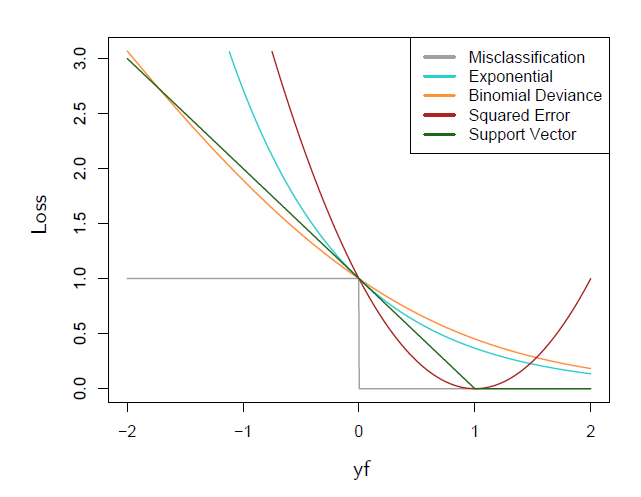
\includegraphics[width=5cm,clip]{images/RobustnessClassification.png}
        \end{figure}
      \end{column}
    \end{columns}
  \end{frame}
  \begin{frame}{回帰における頑健さ}
    \begin{columns}[t]
      \begin{column}{0.5\linewidth}
        \begin{itemize}
          \item 回帰では, 損失関数は残差$y-f(x)$の関数として定めればよい.
          \item Squared-errorは平均, 残差の絶対値は中央値と対応することは前にまとめた通り.

          中央値の方が頑健であることもすぐに分かる.

          \item 中央値の頑健さとSquared-errorの滑らかさを両立させる方法として, ``Huber loss''というものがある.

          一定範囲外は直線, 範囲内は放物線.
        \end{itemize}
      \end{column}
      \begin{column}{0.5\linewidth}
        \begin{figure}[htb]
          \centering
          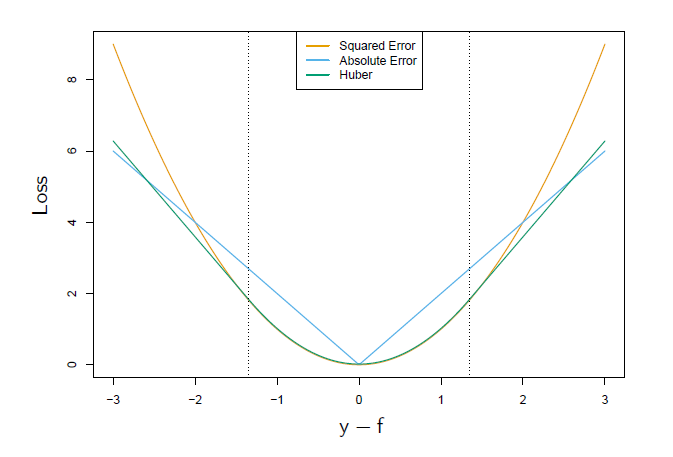
\includegraphics[width=5cm,clip]{images/RobustnessRegression.png}
        \end{figure}
      \end{column}
    \end{columns}
  \end{frame}
  \begin{frame}{頑健さと扱いやすさ}
    以上を踏まえると, 回帰においてSquared-errorを使ったり, 分類において指数損失を使うのは, 頑健さの観点から, 微妙なチョイス.

    一方で, これらはとても計算しやすい.
    (双方, Forward Stagewiseの1周期分の計算が非常に簡潔になる. )

    → 頑健さと扱いやすさを両立した方法を考えられないか?
    → 単純に損失関数を頑健なものに変えるだけではできないので, 後の節で考えます.
  \end{frame}
  \section{Data Mining における手法の``実用性''の話\\p.350-}
  \begin{frame}{実用性の観点と比較}
    \begin{columns}[t]
      \begin{column}{0.3\linewidth}
        \begin{itemize}
          \item 入力値の形式が色々でも耐えるか. (numerical, binary, categorical)
          \item 欠損値
          \item 外れ値
          \item 入力値の単調変換
          \item 計算量
          \item 実は意味のなかった入力変数
          \item 入力変数の合体(PCAのイメージ)
          \item 結果の解釈しやすさ
          \item 予測能力
        \end{itemize}
      \end{column}
      \begin{column}{0.7\linewidth}
        \begin{figure}[htb]
          \centering
          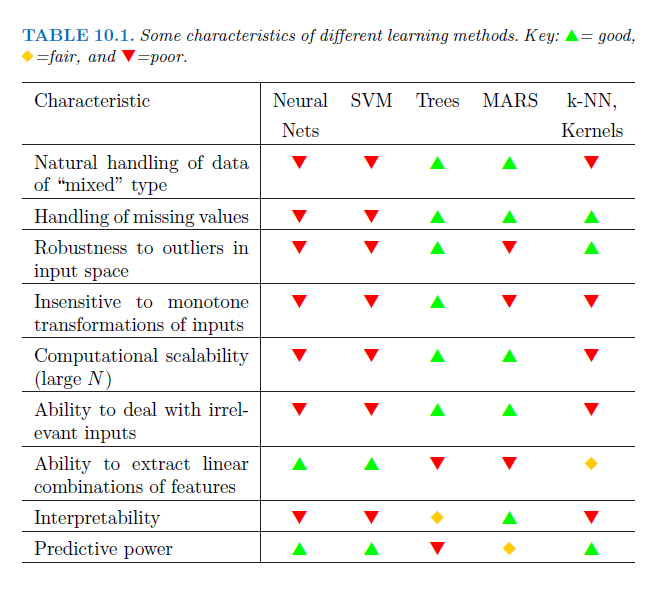
\includegraphics[width=7cm,clip]{images/OffTheShelf.png}
        \end{figure}
      \end{column}
    \end{columns}
  \end{frame}
  \begin{frame}{実用性の観点と比較}
    \begin{columns}[t]
      \begin{column}{0.5\linewidth}
        \begin{itemize}
          \item 決定木は, 予測能力以外とても良い方法.
          \item 決定木を使ってBoostingすれば, 予測能力を向上出来ていい感じ.
          \item 計算量, 解釈しやすさが多少犠牲になる.
          \item これらの犠牲をさらに減らす方法として, 勾配Boostingが考えられている.
        \end{itemize}
      \end{column}
      \begin{column}{0.5\linewidth}
        \begin{figure}[htb]
          \centering
          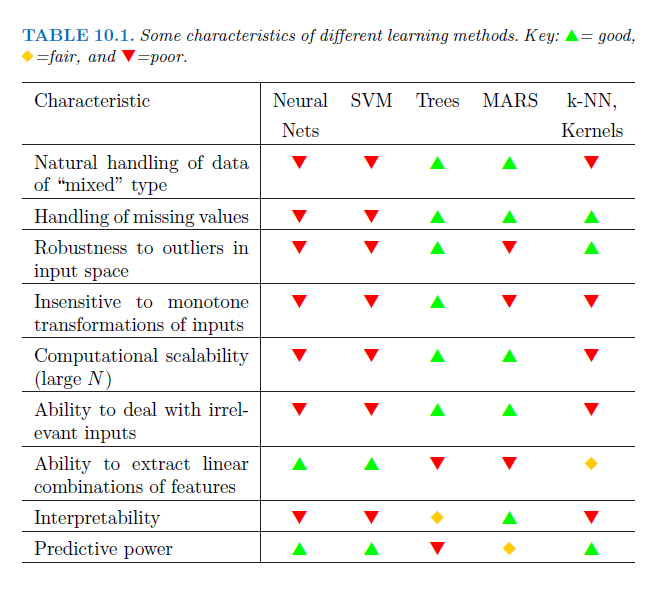
\includegraphics[width=5cm,clip]{images/OffTheShelf.png}
        \end{figure}
      \end{column}
    \end{columns}
  \end{frame}
  \section{木を使ったBoostingの話\\p.353-}
  \begin{frame}{木の表現}
    木$T$は階段関数と思えた. つまり, 入力変数の空間のMECEな分割$R_{j} \ (j=1,\dots,J)$と実数$\gamma_{j}$によって
    \[
      x\in R_{j} \Rightarrow T(x)=\gamma_{j}
    \]
    と定められる. より形式的に書くと, $\Theta=\{R_{j}, \gamma_{j}\}_{j=1}^{J}$をパラメータとして,
    \[
      T(x;\Theta)=\sum_{j=1}^{J}\gamma_{j}I(x\in R_{j})
    \]
    と書ける.
  \end{frame}
  \begin{frame}{木の最適化}
    最適なパラメータを見つけたい. 普通に考えると, 以下を計算したくなる.
    \[
      \hat{\Theta}=\mathrm{arg}\min_{\Theta}\sum_{j=1}{J}\sum_{x_{i} \in R_{j}}L(y_{i}, \gamma_{i})
    \]
    でも, こんなの計算量が多すぎる. どうしたらいいか. 最適化の計算を以下のように整理する.
    \begin{description}
      \item[Step.1] $R_{j}$を固定して, $\gamma_{j}$を最適化する. 大抵簡単な計算. 平均とか, 最頻値とか.
      \item[Step.2] Step.1の結果を使って, $R_j$を決定する. 大抵難しいので, 近似の出番.
    \end{description}
    Step.2での近似として良くやるのは, 貪欲法. また, 損失関数をもっと計算しやすいものに変えることもしばしば. (ようわからん. やってみないと旨味が感じられなそう. )
    \[
      \tilde{\Theta}=\mathrm{arg}\min_{\Theta}\sum_{j=1}{J}\sum_{x_{i} \in R_{j}}\tilde{L}(y_{i}, \gamma_{i})
    \]
    $\hat{R_{j}}=\tilde{R_{j}}$として, $\gamma_{j}$の値の決定時には, 元の損失関数を使う.
  \end{frame}
  \begin{frame}{木でBoosting}
    木でBoostingする場合, $m$回目の最適化では以下を最小化する.
    \[
      \hat{\Theta}_{m}=\mathrm{arg}\min_{\Theta_{m}}\sum_{i=1}^{N}L(y_i,f_{m-1}(x_i)+T(x_i;\Theta_{m})
    \]
    ただし, $f_{m}$は$m$回目の最適化の結果で, 木の和
    \[
      f_{m}(x)=\sum_{k=1}^{m}T(x;\Theta_{k})
    \]
    とする. 先述の通り, この最適化はとても大変. 何ならただの木の最適化より大変な場合もある. だけど, 楽にできるケースもある.
  \end{frame}
  \begin{frame}{木でBoostingが楽なケース}
    \begin{itemize}
      \item 損失関数がSquared-errorの場合.

      各ステップの最適化は, 通常の木の最適化と全く同じ.

      \item 2値分類で指数損失関数を使う場合.

      AdaBoost. 特に$\gamma_{jm} \in \{-1,1\}$の時, 損失の最小化は, 重み付き誤差率
      \[
        \sum_{i=1}^{N}e^{-y_if_{m-1}(x_i)}\dot e^{-y_iT(x_i;\Theta_m)}
      \]
      の最小化と等価.

      \item 一方, 頑健さのために, 損失関数として絶対値誤差, Huber loss, deviance等を使うと, 頑健さは改善するが, 上記のような単純な計算に落とし込めなくなる.

      \item 一般論として, 領域の分割方法さえ決まれば, パラメータ$\gamma$は比較的容易に求まる. 領域を決めることは非常に困難で, 良い近似手法を考えることが重要.
    \end{itemize}
  \end{frame}
  \section{勾配Boostingの話\\p.358-}
  \begin{frame}{最急降下法}
    関数の最小値を発見する手法. これを応用して木の最適化を考えていく.
    \begin{itemize}
      \item 最も傾斜が急な方向に最も小さくなる位置まで移動する, という処理を繰り返して最小点を探す手法. 貪欲法.
      \item 関数$f(x_1,\dots,x_n)$の最小化を考えるとすると, $\textbf{x}^{(0)}$を適当にとって, $m=1,2,\dots$に対して, 収束するまで以下を繰り返す.
      \begin{enumerate}
        \item 方向を決める. 勾配ベクトルの逆方向なので勾配(gradient)を計算すればよい.         \[
          g_m=\mathrm{grad}f(\textbf{x}_i)=\frac{\partial f}{\partial x_i}(\textbf{x}^{(m)})
        \]
        \item 距離を決める.
        \[
          \rho_m=\mathrm{arg}\min_{\rho}f(\textbf{x}^{(m)}-\rho g_m)
        \]
        \item 値を更新する.
        \[
          \textbf{x}^{(m+1)}=\textbf{x}^{(m)}-\rho g_m
        \]
      \end{enumerate}
    \end{itemize}
  \end{frame}
  \begin{frame}{勾配Boosting}
    さっきの話を木の最適化に使いたい. 損失関数の合計
    \[
      L(f)=\sum_{i=1}^{N}L(y_i,f(x_i))
    \]
    の最小化なので, この値を$\textbf{f}={f(x_i)}_{i=1}^{N}$の関数とみなして, 最急降下法を使いたい. が, そのまま適用はできない. 問題点は以下.
    \begin{itemize}
      \item 最急降下法では入力値$\textbf{x}$に制約はないが, 上記のように定めた$\textbf{f}$は高々$J_m$種類の値しか含まない.
      \item 最急降下法では, 向きを完全に決めてから距離を決めるが, 木の最適化では, 領域の分割を決めてから各領域ごとに独立に高さを計算する.
      \item 勾配は訓練データに対する値しか考慮していないので, 過学習を防げない.
    \end{itemize}
    ここら辺の差異を避けて, 最急降下法の肝だけを活用する方法として, 次の方法が挙げられる. (汎化性能の問題解決できてないのでは...??)
    \begin{itemize}
      \item 領域の決定のために, 勾配ベクトルとの残差二乗和を最小化する木を見つける.
      \[
        \hat{\Theta}_m=\mathrm{arg}\min_{\Theta}\sum_{i=1}^{N}(-g_{im}-T(x_i;\Theta))^2
      \]
      \item これで定まる各領域$R_{jm}$について, 良い$\gamma_{jm}$の値を計算する.
    \end{itemize}
    この2段階は, まさしくさっき言ったもの.
  \end{frame}
  \begin{frame}{勾配Boostingの実装}
    \begin{columns}[t]
      \begin{column}{0.5\linewidth}
        \begin{itemize}
          \item 勾配Boostingで回帰するアルゴリズム.
          \item 2-(b)で領域の分割決定.
          \item 2-(c)で各領域に対応する$\gamma$の値を決定.
          \item 分類についても似たようなもん. 多値分類の場合, 繰り返しの回数は$M \dot (\mbox{クラス数})$回.
        \end{itemize}
      \end{column}
      \begin{column}{0.5\linewidth}
        \begin{figure}[htb]
          \centering
          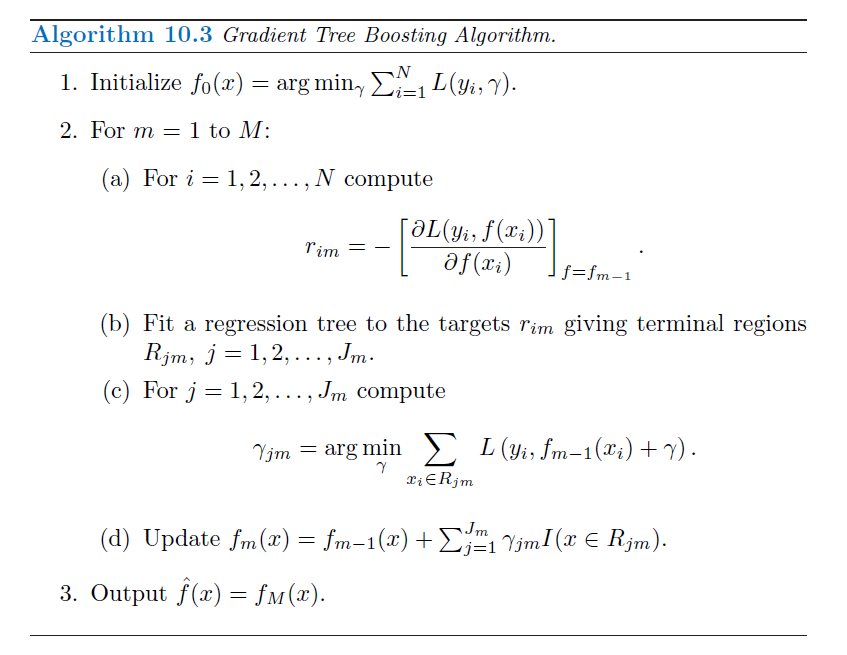
\includegraphics[width=5cm,clip]{images/GradientBoosting.png}
        \end{figure}
      \end{column}
    \end{columns}
  \end{frame}
  \begin{frame}{勾配Boostingのメタパラメータその1:木のサイズ$J$}
    \textbf{普通木を作るときの決め方}
    \begin{itemize}
      \item 普通の木では, 大きく作って刈り込む作戦がとられたり.
      \item 刈り込みをする時点で, 「最適な分類」をしようとするので, Boostingで使うと, 不必要に強いものが残りがち.
      \item 結果, 過剰な計算量と大きすぎる木たち, ということになりがち.
    \end{itemize}
    \textbf{最も単純な回避策}
    \begin{itemize}
      \item すべての木のサイズを同じ値$J_m=J \ \forall m$にして, $J$を調整する.
      \item この$J$は, モデル自体の変数(メタパラメータ, ハイパーパラメータ)と思える.
      (基底関数展開の基底の数やk-NNのkみたいな)
    \end{itemize}
    \textbf{Jの値の決め方}
    \begin{itemize}
      \item 前に出てきたANOVA分解.
      \[
        \eta(X)=\sum_i\eta_i(X_i)+\sum_{i,j}\eta_{i,j}(X_i,X_j)+\cdots
      \]
      \item 入力変数の交互作用の程度を考える. 大きさ$J$の木で起こる交互作用は高々$J-1$.
      \item 交互作用の程度は, 大抵それほど多くない. 経験的に, $J>10$が必要なことはほぼない. $4 \le J \le 8$程度がうまくいく.
    \end{itemize}
  \end{frame}
  \section{正則化の話\\p.364-}
  \begin{frame}{勾配Boostingのメタパラメータその2:Boostingの回数$M$}
    \begin{itemize}
      \item $M$を増やすほど損失は減るが, やりすぎると過学習.
      \item 丁度良い$M$の値を見つけなくてはいけない.
      \item 検証用データを別に用意するのは良くある戦略.
      \item Neural Networkのearly stoppingとよく似ているとか. (11章で見る. )
    \end{itemize}
    過学習を防ぐ方法として, $M$の値を操作する以外の方法もある.
  \end{frame}
  \begin{frame}{過学習を防ぐ方法1:縮小法}
    \begin{itemize}
      \item $M$ではなく, アルゴリズムをちょっといじって, 過学習を防ぐ方法.
      \item $f_m$の更新時に係数をかけて, 更新幅を縮小する.
      \[
        f_m(x)=f_{m-1}+\nu\sum_{j=1}^J\gamma_{jm}I(x\in R_{jm})
      \]
      \item $\nu$が学習率をコントロールしている. 小さいほど学習率が低い.
      \item 経験的に, $\nu$を小さく($\le 1$とか)とり, $M$はearly stoppingすることで, いい感じにできる. 特に回帰では効果的.
      \item ただし, 計算量は増える.
    \end{itemize}
  \end{frame}
  \begin{frame}{縮小法の結果}
    \begin{figure}[htb]
      \centering
      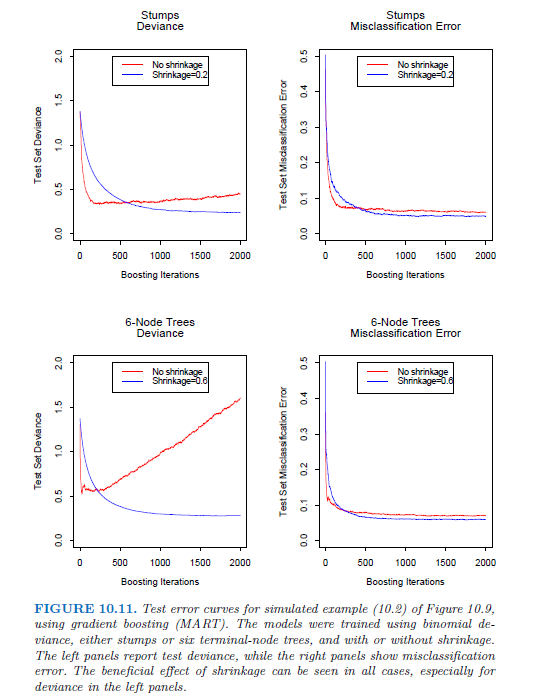
\includegraphics[width=8cm,clip]{images/Shrinkage.png}
    \end{figure}
  \end{frame}
  \begin{frame}{過学習を防ぐ方法2:部分標本}
    \begin{columns}[t]
      \begin{column}{0.5\linewidth}
        \begin{itemize}
          \item bootstrap法に似た考え方を使う.
          \item 繰り返しのたびに, 訓練データから一定数のデータを非復元抽出して, そのデータを使って最適化する.
          \item 「一定数」は, 訓練データの半数程度が相場. $N$が大きければもっと少なくてもよい.
          \item 計算量はもちろん改善. 多くの場合, 精度も良くなる.
          \item 右図から, 部分標本と縮小法を併用したときが最も良いことが分かる.
        \end{itemize}
      \end{column}
      \begin{column}{0.5\linewidth}
        \begin{figure}[htb]
          \centering
          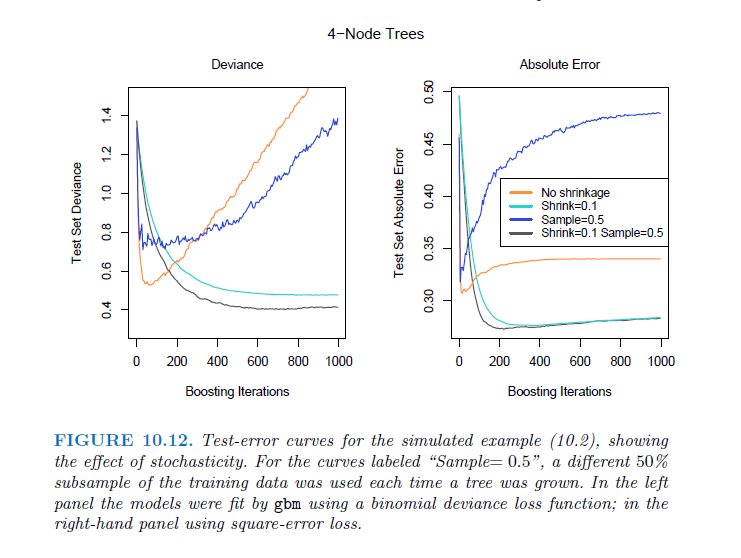
\includegraphics[width=5cm,clip]{images/Subsampling.png}
        \end{figure}
      \end{column}
    \end{columns}
  \end{frame}
  \section{計算結果の解釈の話\\p.367-}
  \begin{frame}{入力変数の相対的な重要さ}
    変数の重要さ
    \begin{itemize}
      \item 入力変数のうち, 一部のみが出力変数に大きな影響を与えていることが多い.
      \item この, ``影響度''の大きさを推定することはとても有用.
    \end{itemize}
    単体の木における入力変数の重要さ
    \begin{itemize}
      \item 以下の式で表されたり.
      \[
        \mathcal{I}_l^2=\sum_{t=1}^{J-1}\hat{i}_t^2I(v(t)=l)
      \]
      \item $\hat{i}_t^2$はその分割における誤差の改善幅.
      \item これはつまり, 木の中でその変数が分割に使われている部分でどれだけ予測が改善したか, ということ.
    \end{itemize}
    木の和への一般化
    \begin{itemize}
      \item 単純に各木における重要さの平均
      \[
        \mathcal{I}_l^2=\frac{1}{M}\sum_{m=1}^M\mathcal{I}_l^2(T_m)
      \]
      \item K値分類の場合, K個の木の和が作られるので, さらにそれらにおける重要度の平均を取る.
    \end{itemize}
  \end{frame}
  \begin{frame}{一部の入力変数の集合の重要さ}
    各変数ごとの重要さの次は, いくつかの入力変数からなる集合の重要さ(部分依存, partial dependence))を考えたい.
    \begin{itemize}
      \item グラフなどで視覚化すると, 分かりやすい. が, 高次元では難しい.
      \item Trellisなど数次元くらいのデータのうまい可視化の仕方もある. けど限界があるよね.
    \end{itemize}
    一部の入力変数の集合の重要さ
    \begin{itemize}
      \item $X_s \subset X$, $X_c=X\backslash X_s$とする.
      \item $f(X)=f(X_s,X_c)$と思える.
      \item $f_s(X_s)=E_{X_c}[f(X_s,X_c)]$とすると, 部分依存を表現できそう.
      実際, $X_s$と$X_c$の間の交互作用が弱いなら, かなりいい.
      \item 母集団に対する値は難しいので, 以下で推定する.
      \[
        \bar{f}_s(X_s)=\frac{1}{N}\sum_{i=1}^Nf(X_s,x_{ic})
      \]
      \item この計算は一般にはすごく大変だけど, $f$が木の時は簡単にできる.
    \end{itemize}
  \end{frame}
  \begin{frame}{部分依存は, 条件付き期待値を使わない}
    \begin{itemize}
      \item 条件付き期待値は, $X_c$の周辺分布を使って平均を計算する.
      \item 一方, 部分依存関数$f_s(X_s)=E_{X_c}[f(X_s,X_c)]$は, 変数$X_c$の全域的な分布を使って計算している.
      \item $X_s$と$X_c$が独立なときのみ, 両者は一致する.
      \item $X_s$と$X_c$について, $f$が完全に加法的なとき, 部分依存関数は$X_s\mbox{部分}+\mbox{定数}$, 乗法的なときは, $X_s\mbox{部分} \times \mbox{定数}$
      \item 条件付き期待値ではそうきれいにはならない.
      \item (だから何なのか良く分からん.
      \item この話もK値分類に拡張できるよ.
    \end{itemize}
  \end{frame}
  \section{残りの部分は具体例だったので飛ばします. おわり. }
\end{document}
